% !TEX root = ../main.tex
\begin{figure}[t]
\vspace{-0.7in}
\begin{minipage}[c]{0.5\linewidth}
\centering
\vspace{0.25in}
\iflatexml
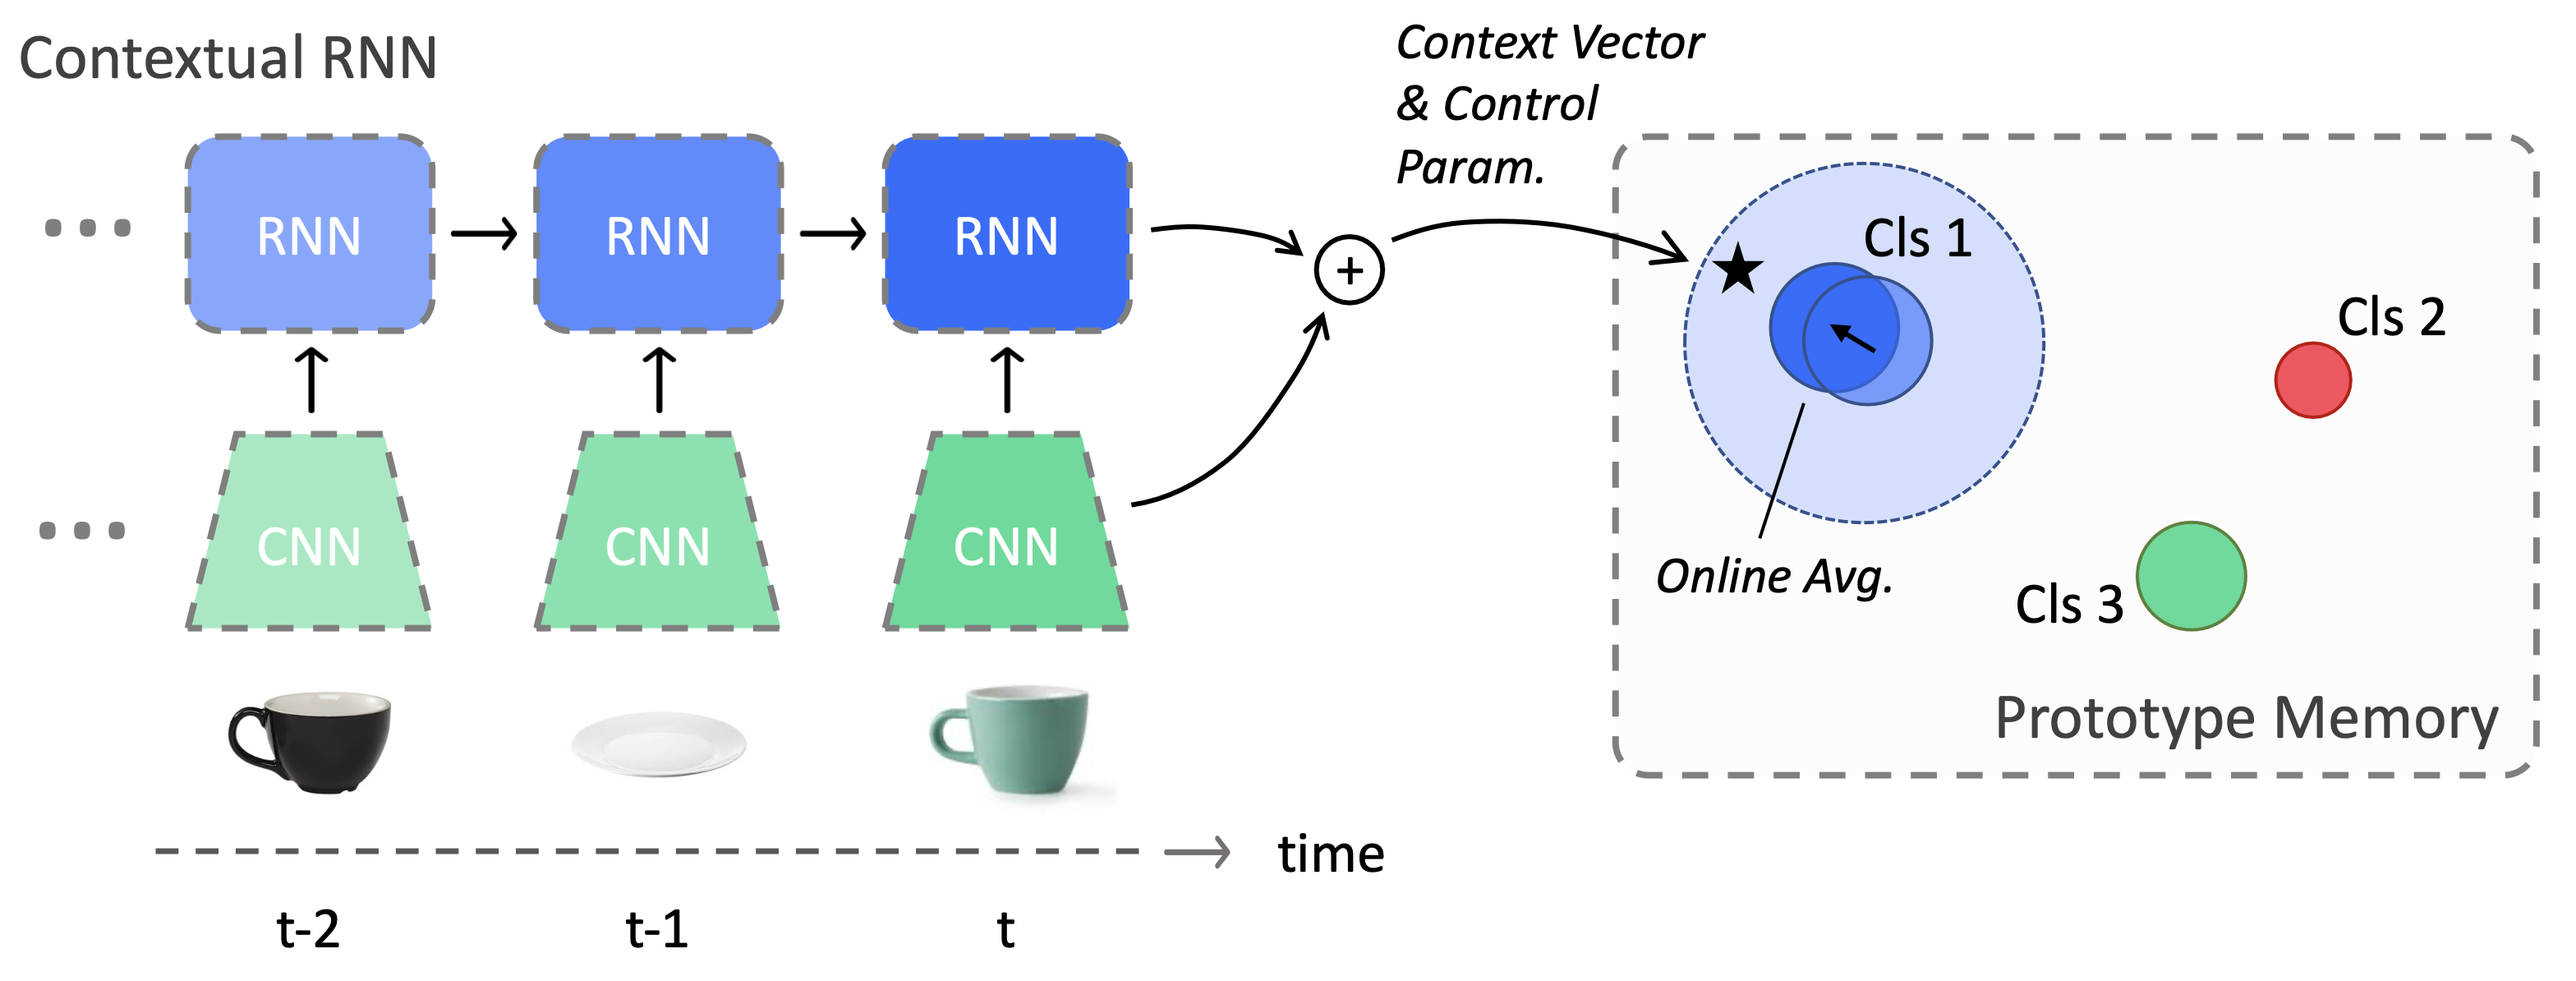
\includegraphics[width=6\linewidth]{figures/our_model.png}
\else
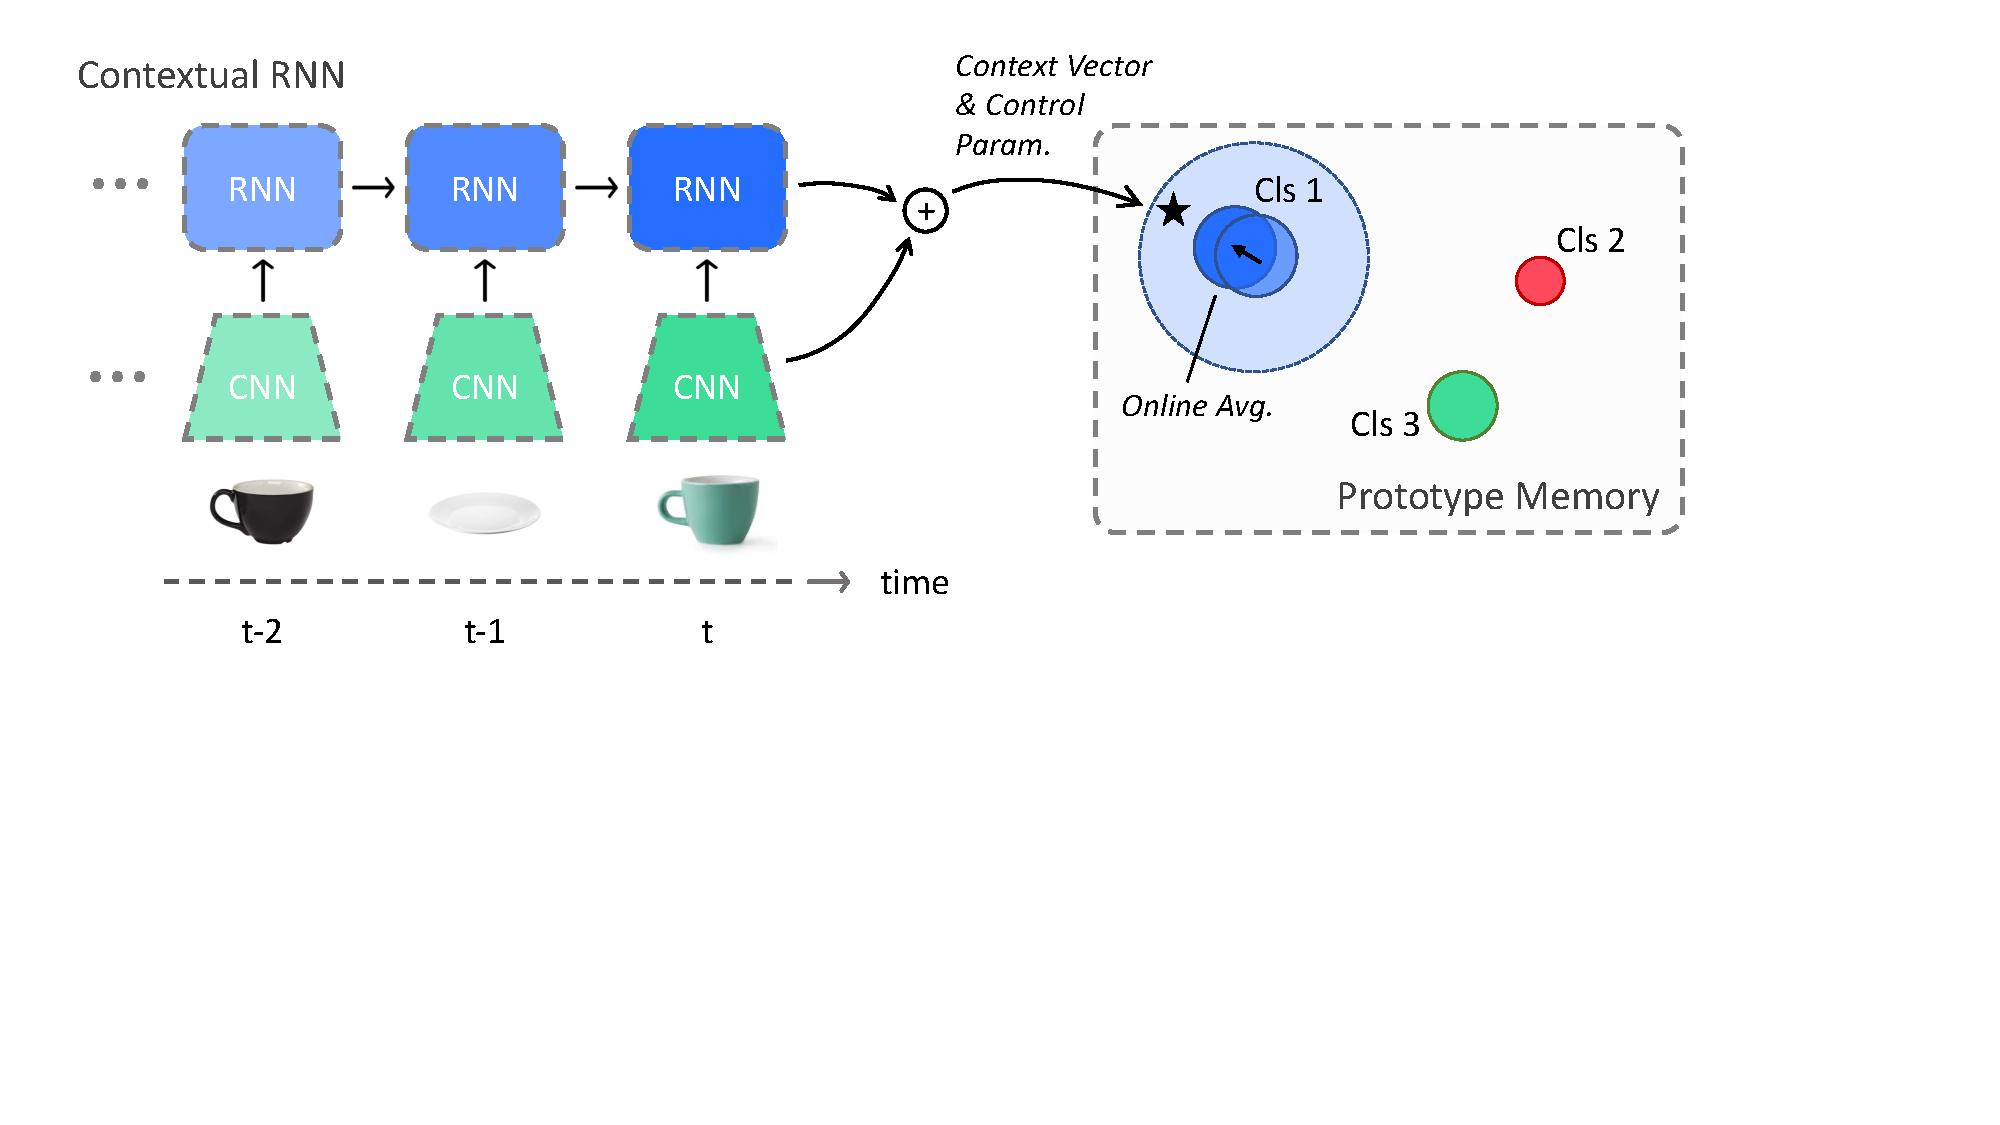
\includegraphics[width=\linewidth,trim={0 8cm 4.5cm 0.3cm},clip]{figures/our_model.pdf}
\fi
\end{minipage}
% \hfill
\begin{minipage}[c]{0.5\linewidth}
\caption{\textbf{Contextual prototypical memory.} Temporal contextual features are extracted
from an RNN. The prototype memory stores one vector per class and does online averaging.
Examples falling outside the radii of all prototypes are classified as ``new.'' }
\label{fig:mainmodel}
\end{minipage}
\vspace{-0.25in}
\end{figure}
